% --------------------------------------------------------------------------------

\begin{exercise}[Sum and average]

Let $X$ be a random variable with $\mathcal{N}(5,2^2)$. Let $X_1,X_2,\dots,X_{50}$
be independent identically distributed copies of $X$. Let $S$ be their sum and $\bar{X}$
their average, i.e.

\begin{align*}
  S = X_1 + \dots + X_{50} \quad \text{and} \quad \bar{X} = \frac{1}{50}(X_1 + \dots + X_{50}).
\end{align*}

\begin{enumerate}[label = (\alph*)]
  \item Plot the density and the distribution function for $X$ using \textsc{R}.
  \item What are the expectation and the standard deviation of $S$ and of $\bar{X}$?
  \item Generate a sample of 50 numbers from $\mathcal{N}(5,2^2)$. Plot the histogram
  for this sample. Do the same for a sample of 500 numbers from $\mathcal{N}(5,2^2)$.
\end{enumerate}

\end{exercise}

% --------------------------------------------------------------------------------

\begin{solution}

\phantom{}

\begin{enumerate}[label = (\alph*)]
  \item
  \begin{figure}[H]
      \centering
      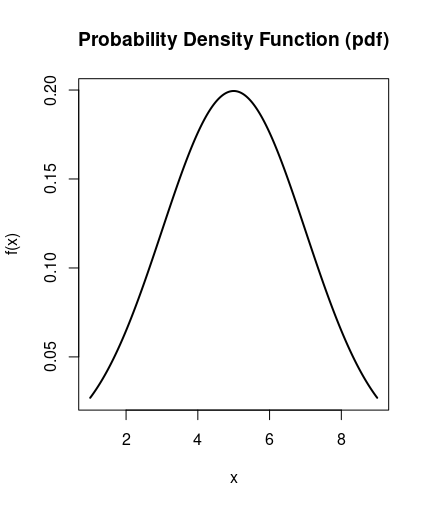
\includegraphics[width = 0.75 \textwidth]{pdf_plot.png}
      \caption{}
      \label{}
  \end{figure}
  \begin{figure}[H]
      \centering
      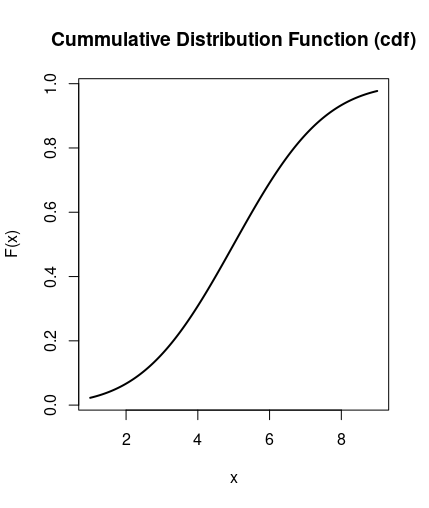
\includegraphics[width = 0.75 \textwidth]{cdf_plot.png}
      \caption{}
      \label{}
  \end{figure}
  \item
  \begin{align*}
    \E(S) &= \E(\sum_{i=1}^{50} X_i) = \sum_{i=1}^{50}5 = 250. \\
    \V(S) &= \V(\sum_{i=1}^{50} X_i) = \sum_{i=1}^{50}4 = 200. \\
    \E(\bar{X}) &= \frac{1}{50}\E(S) = 5. \\
    \V(\bar{X}) &= \frac{1}{50}\V(S) = 0.08.
  \end{align*}
  \item
  \begin{figure}[H]
      \centering
      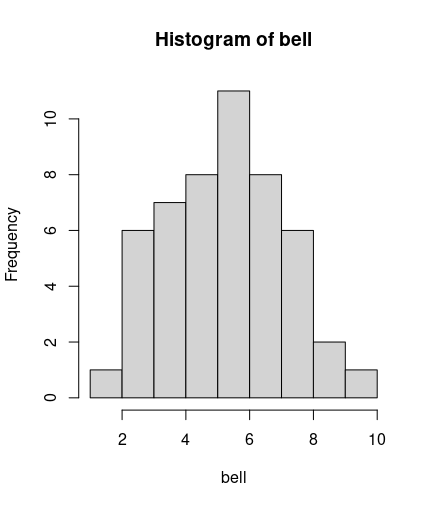
\includegraphics[width = 0.75 \textwidth]{hist_1.png}
      \caption{}
      \label{}
  \end{figure}
  \begin{figure}[H]
      \centering
      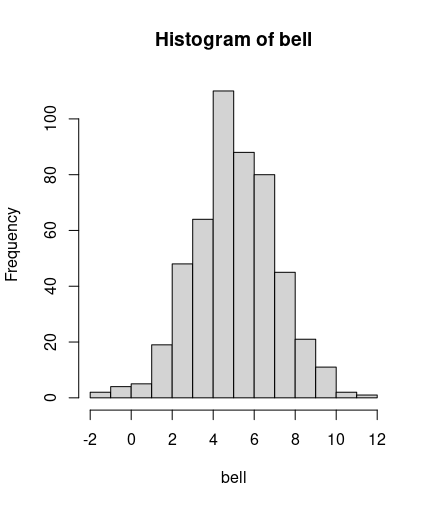
\includegraphics[width = 0.75 \textwidth]{hist_2.png}
      \caption{}
      \label{}
  \end{figure}
\end{enumerate}

\end{solution}

% --------------------------------------------------------------------------------
